\documentclass[11pt, a4paper]{article}
\usepackage[UTF8]{ctex} % For Chinese character support
\usepackage{geometry}
\usepackage{graphicx}
\usepackage{amsmath}
\usepackage{amssymb}
\usepackage{enumitem} % For customized lists
\usepackage{hyperref} % For hyperlinks
\usepackage{xcolor}   % For colors
\usepackage{listings} % For code listings
\usepackage{caption}  % For captions
\usepackage{titling} % Add this line for title customization

% Page geometry
\geometry{a4paper, margin=1in}

% Listings style for SQL
% In your LaTeX preamble (e.g., where other \lstdefinestyle commands are)
\lstdefinestyle{sqlstyle}{
    language=SQL,
    basicstyle=\ttfamily\footnotesize,
    keywordstyle=\color{blue}\bfseries,
    stringstyle=\color{red!60!black},
    commentstyle=\color{green!60!black},
    morecomment=[l]--,%           SQL comments
    numbers=left,
    numberstyle=\tiny\color{gray},
    breaklines=true,
    breakatwhitespace=true,
    tabsize=2,
    captionpos=b, % caption below
    extendedchars=true,
    showstringspaces=false, % <--- CRITICAL FIX: Add this line
    literate={--}{{-{}-}}2 % to display double hyphen correctly
}

% Add this to your LaTeX preamble, for example, after the \lstdefinestyle{sqlstyle}
\lstdefinestyle{pythonstyle}{
    language=Python,
    basicstyle=\ttfamily\footnotesize,
    keywordstyle=\color{blue}\bfseries,      % Keywords
    stringstyle=\color{red!60!black},        % Strings
    commentstyle=\color{green!60!black},     % Comments
    identifierstyle=\color{black},           % Other identifiers
    emph={self,True,False,None,def,class,import,from,return,if,elif,else,for,while,try,except,finally,with,as,in,is,not,and,or,pass,global,nonlocal,yield,assert,break,continue,del,lambda}, % Python keywords
    emphstyle=\color{blue}\bfseries,          % Style for keywords in emph
    emph={[2]request,render_template,redirect,url_for,flash,g,current_app,Flask,os,psycopg2,app,db,click,load_dotenv}, % Common Flask/library names
    emphstyle={[2]\color{teal}\bfseries},       % Style for emph[2]
    numbers=left,
    numberstyle=\tiny\color{gray},
    breaklines=true,
    breakatwhitespace=true,
    tabsize=4,
    captionpos=b,
    extendedchars=true, % Important for UTF-8 characters in comments/strings
    showstringspaces=false, % Don't show spaces in strings with special characters
    literate={->}{{$\rightarrow$}}1 {!=}{{$\neq$}}1 {<=}{{$\leq$}}1 {>=}{{$\geq$}}1, % Ligatures
}

% Hyperref setup
\hypersetup{
    colorlinks=true,
    linkcolor=blue,
    filecolor=magenta,
    urlcolor=cyan,
    pdftitle={个人图书管理系统设计},
    pdfpagemode=FullScreen,
}

% Add these lines to left-align the title
\pretitle{\begin{flushleft}\LARGE\bfseries}
\posttitle{\end{flushleft}}

\title{实验二:小型图书管理系统}
\date{}

\begin{document}
\maketitle

\section{系统功能需求}
本个人图书管理系统旨在提供一个便捷的平台,用于管理个人藏书、读者信息以及图书的借阅和归还过程。系统应具备以下主要功能:

\begin{enumerate}
    \item \textbf{图书管理 (Books Management)}
    \begin{itemize}
        \item \textbf{添加图书}: 管理员能够向系统中添加新的图书信息,包括书名、作者、ISBN(国际标准书号,具有唯一性)、出版社、出版年份、分类、总库存量。添加时,可借阅库存默认为总库存。
        \item \textbf{编辑图书}: 管理员能够修改已存在的图书信息,包括上述所有字段。修改库存时,需确保可借阅库存不大于总库存,且两者均不能为负数。
        \item \textbf{删除图书}: 管理员能够从系统中删除图书。如果图书当前有未归还的借阅记录,则不允许删除,并提示用户。
        \item \textbf{查询与浏览图书}:
        \begin{itemize}
            \item 用户可以浏览所有图书的列表,列表应包含关键信息(如书名、作者、ISBN、分类、总库存、可借阅库存)。
            \item 支持分页显示图书列表,以优化大量数据时的浏览体验。
            \item 支持按书名、作者或 ISBN 进行模糊搜索或精确搜索。
        \end{itemize}
        \item \textbf{查看图书详情}: 能够查看单本图书的完整详细信息。
    \end{itemize}

    \item \textbf{读者管理 (Readers Management)}
    \begin{itemize}
        \item \textbf{添加读者}: 管理员能够添加新的读者信息,包括姓名、读者编号、联系方式。
        \item \textbf{编辑读者}: 管理员能够修改已存在的读者信息。
        \item \textbf{删除读者}: 管理员能够删除读者。如果读者当前有未归还的图书,则不允许删除,并提示用户。
        \item \textbf{查询与浏览读者}: 用户可以浏览所有读者的列表,列表应包含关键信息(如姓名、读者编号、联系方式)。
    \end{itemize}

    \item \textbf{借阅管理 (Loans Management)}
    \begin{itemize}
        \item \textbf{借书}:
        \begin{itemize}
            \item 管理员能够为指定读者借阅指定的图书。
            \item 借书时需选择图书和读者,并指定应归还日期。
            \item 系统自动记录借阅日期为当前日期。
            \item 借书成功后,对应图书的“可借阅库存”会自动减 1。
            \item 如果图书的可借阅库存为 0,则不允许借阅。
            \item 借书操作应在一个数据库事务中完成,确保数据一致性。
        \end{itemize}
        \item \textbf{还书}:
        \begin{itemize}
            \item 管理员能够记录指定借阅记录的归还操作。
            \item 还书时,系统自动记录归还日期为当前日期。
            \item 还书成功后,对应图书的“可借阅库存”会自动加 1。
            \item 还书操作应在一个数据库事务中完成。
        \end{itemize}
        \item \textbf{查询当前借阅}: 用户可以查看所有当前未归还的借阅记录列表,包括借阅的图书信息、读者信息、借阅日期和应归还日期。
        \item \textbf{查询逾期借阅}: 用户可以查看所有已到期但尚未归还的借阅记录列表,以便进行催还。
    \end{itemize}

    \item \textbf{综合查询 (Comprehensive Search/Reports)}
    \begin{itemize}
        \item \textbf{查询读者借阅历史}: 用户可以根据读者查询其所有的借阅历史记录(包括已归还和未归还的)。
        \item \textbf{查询图书借阅历史}: 用户可以根据图书查询其所有的被借阅历史记录。
    \end{itemize}

    \item \textbf{系统层面}
    \begin{itemize}
        \item \textbf{数据库初始化}: 提供命令行工具,用于初始化数据库表结构及预定义的视图和触发器。
        \item \textbf{用户界面}: 提供简洁易用的 Web 用户界面,方便用户进行各项操作。
        \item \textbf{错误提示与反馈}: 对用户的操作提供明确的成功或失败提示,对错误操作(如输入不合法、违反约束等)给出清晰的错误信息。
    \end{itemize}
\end{enumerate}

\newpage
\section{数据库设计}

\subsection{E-R 图设计及其说明}
\subsubsection*{实体 (Entities)}
根据系统需求,我们识别出以下主要实体:
\begin{itemize}
    \item \textbf{读者 (Reader)}: 存储读者的基本信息。
    \item \textbf{图书 (Book)}: 存储图书的详细信息。
    \item \textbf{借阅 (Loan)}: 记录图书的借阅活动,连接读者和图书。
\end{itemize}

\subsubsection*{关系 (Relationships)}
\begin{itemize}
    \item 一个 \textbf{读者} 可以有多条 \textbf{借阅} 记录 (一对多关系: Reader 1 --- * Loan)。
    \item 一本 \textbf{图书} 可以有多条 \textbf{借阅} 记录 (一对多关系: Book 1 --- * Loan)。
    \begin{itemize}
        \item 因此,\textbf{借阅 (Loan)} 实体是一个关联实体,它解决了 \textbf{读者 (Reader)} 和 \textbf{图书 (Book)} 之间的多对多关系(一个读者可以借阅多本书,一本书可以被多个读者借阅)。
    \end{itemize}
\end{itemize}

\subsubsection*{属性 (Attributes)}
\begin{itemize}
    \item \textbf{读者 (Reader)}: \texttt{reader\_id} (主键), \texttt{name}, \texttt{reader\_number} (唯一), \texttt{contact}
    \item \textbf{图书 (Book)}: \texttt{book\_id} (主键), \texttt{title}, \texttt{author}, \texttt{isbn} (唯一), \texttt{publisher}, \texttt{publication\_year}, \texttt{category}, \texttt{total\_stock}, \texttt{available\_stock}
    \item \textbf{借阅 (Loan)}: \texttt{loan\_id} (主键), \texttt{book\_id} (外键), \texttt{reader\_id} (外键), \texttt{loan\_date}, \texttt{due\_date}, \texttt{return\_date}
\end{itemize}

\subsubsection*{E-R 图 (Conceptual)}
\begin{figure}[htbp]
    \centering
    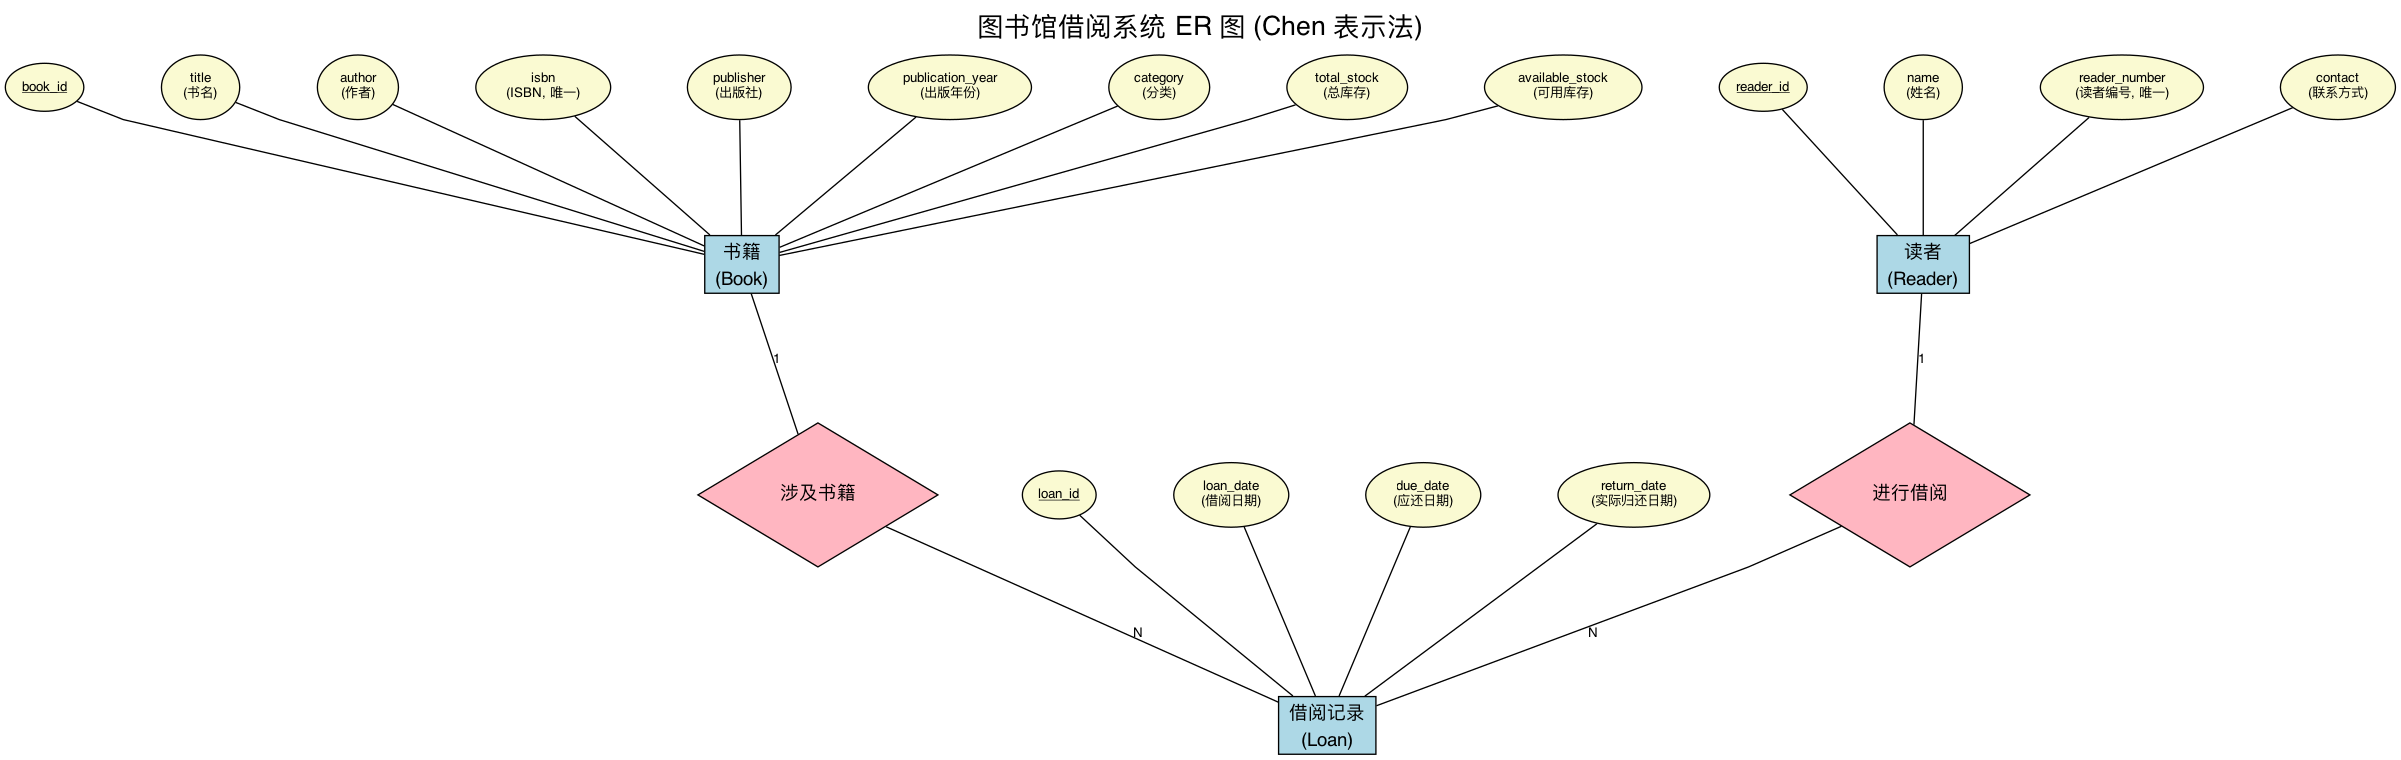
\includegraphics[width=0.8\textwidth]{library_chen_er_diagram.png} % Make sure this image file exists
    \caption{个人图书管理系统 E-R 图}
    \label{fig:er_diagram}
\end{figure}

\subsection{数据库逻辑结构设计}
数据库包含三个主要表:\texttt{readers}, \texttt{books}, 和 \texttt{loans},以及两个视图 \texttt{view\_activeloans} 和 \texttt{view\_overdueloans}。这些结构定义在 \texttt{personal\_library/schema.sql} 文件中。

\subsubsection{表结构}
\paragraph{\texttt{readers} 表}
\begin{itemize}
    \item \textbf{说明}: 存储读者信息。
    \item \textbf{逻辑结构}:
    \begin{itemize}
        \item \texttt{reader\_id}: \texttt{SERIAL}, 主键 (PK)。自动递增的唯一标识符。
        \item \texttt{name}: \texttt{VARCHAR(100)}, \texttt{NOT NULL}。读者姓名。
        \item \texttt{reader\_number}: \texttt{VARCHAR(50)}, \texttt{UNIQUE}, \texttt{NOT NULL}。读者编号,具有唯一性约束。
        \item \texttt{contact}: \texttt{VARCHAR(100)}。读者联系方式,可为空。
    \end{itemize}
\end{itemize}

\paragraph{\texttt{books} 表}
\begin{itemize}
    \item \textbf{说明}: 存储图书信息。
    \item \textbf{逻辑结构}:
    \begin{itemize}
        \item \texttt{book\_id}: \texttt{SERIAL}, 主键 (PK)。自动递增的唯一标识符。
        \item \texttt{title}: \texttt{VARCHAR(255)}, \texttt{NOT NULL}。图书标题。
        \item \texttt{author}: \texttt{VARCHAR(100)}, \texttt{NOT NULL}。图书作者。
        \item \texttt{isbn}: \texttt{VARCHAR(20)}, \texttt{UNIQUE}, \texttt{NOT NULL}。国际标准书号,具有唯一性约束。
        \item \texttt{publisher}: \texttt{VARCHAR(100)}。出版社,可为空。
        \item \texttt{publication\_year}: \texttt{INTEGER}。出版年份,可为空。
        \item \texttt{category}: \texttt{VARCHAR(50)}。图书分类,可为空。
        \item \texttt{total\_stock}: \texttt{INTEGER}, \texttt{NOT NULL}, \texttt{DEFAULT 0}。总库存量。
        \begin{itemize}
            \item 用户定义完整性: \texttt{CONSTRAINT chk\_total\_stock CHECK (total\_stock >= 0)} 确保总库存不为负。
        \end{itemize}
        \item \texttt{available\_stock}: \texttt{INTEGER}, \texttt{NOT NULL}, \texttt{DEFAULT 0}。可借阅库存量。
        \begin{itemize}
            \item 用户定义完整性: \texttt{CONSTRAINT chk\_available\_stock CHECK (available\_stock >= 0 AND available\_stock <= total\_stock)} 确保可借阅库存不为负且不超过总库存。
        \end{itemize}
    \end{itemize}
\end{itemize}

\paragraph{\texttt{loans} 表}
\begin{itemize}
    \item \textbf{说明}: 存储借阅记录,关联 \texttt{books} 表和 \texttt{readers} 表。
    \item \textbf{逻辑结构}:
    \begin{itemize}
        \item \texttt{loan\_id}: \texttt{SERIAL}, 主键 (PK)。自动递增的唯一标识符。
        \item \texttt{book\_id}: \texttt{INTEGER}, \texttt{NOT NULL}。外键 (FK),参照 \texttt{books(book\_id)}。
        \begin{itemize}
            \item 参照完整性: \texttt{ON DELETE RESTRICT} - 如果某本图书在 \texttt{books} 表中被删除,但其 \texttt{book\_id} 仍存在于 \texttt{loans} 表的未归还记录中,则禁止删除该图书。
        \end{itemize}
        \item \texttt{reader\_id}: \texttt{INTEGER}, \texttt{NOT NULL}。外键 (FK),参照 \texttt{readers(reader\_id)}。
        \begin{itemize}
            \item 参照完整性: \texttt{ON DELETE RESTRICT} - 如果某个读者在 \texttt{readers} 表中被删除,但其 \texttt{reader\_id} 仍存在于 \texttt{loans} 表的未归还记录中,则禁止删除该读者。
        \end{itemize}
        \item \texttt{loan\_date}: \texttt{DATE}, \texttt{NOT NULL}, \texttt{DEFAULT CURRENT\_DATE}。借阅日期,默认为当前日期。
        \item \texttt{due\_date}: \texttt{DATE}, \texttt{NOT NULL}。应归还日期。
        \item \texttt{return\_date}: \texttt{DATE}, \texttt{DEFAULT NULL}。实际归还日期,默认为 \texttt{NULL} (表示未归还)。
    \end{itemize}
\end{itemize}

\subsubsection{视图结构}
\paragraph{\texttt{view\_activeloans} 视图}
\begin{itemize}
    \item \textbf{说明}: 显示所有当前未归还的借阅记录的详细信息。
    \item \textbf{逻辑结构}: 该视图通过连接 \texttt{loans}, \texttt{books}, 和 \texttt{readers} 表,筛选出 \texttt{loans.return\_date} 为 \texttt{NULL} 的记录。
    \begin{itemize}
        \item \texttt{loan\_id}: 借阅ID。
        \item \texttt{reader\_name}: 读者姓名。
        \item \texttt{reader\_number}: 读者编号。
        \item \texttt{book\_title}: 图书标题。
        \item \texttt{isbn}: 图书ISBN。
        \item \texttt{loan\_date}: 借阅日期。
        \item \texttt{due\_date}: 应归还日期。
    \end{itemize}
\end{itemize}

\paragraph{\texttt{view\_overdueloans} 视图}
\begin{itemize}
    \item \textbf{说明}: 显示所有已逾期但尚未归还的借阅记录。
    \item \textbf{逻辑结构}: 该视图基于 \texttt{loans}, \texttt{books}, 和 \texttt{readers} 表,筛选出 \texttt{loans.return\_date} 为 \texttt{NULL} 且 \texttt{loans.due\_date} 早于当前日期的记录。
    \begin{itemize}
        \item \texttt{loan\_id}: 借阅ID。
        \item \texttt{reader\_name}: 读者姓名。
        \item \texttt{reader\_number}: 读者编号。
        \item \texttt{reader\_contact}: 读者联系方式。
        \item \texttt{book\_title}: 图书标题。
        \item \texttt{isbn}: 图书ISBN。
        \item \texttt{loan\_date}: 借阅日期。
        \item \texttt{due\_date}: 应归还日期。
    \end{itemize}
\end{itemize}

\subsection{数据库物理设计}
为了优化查询性能,在数据库表的一些关键列上创建了索引。这些索引定义在 \texttt{personal\_library/schema.sql} 文件中。

\subsubsection{索引定义}
\paragraph{\texttt{books} 表索引}
\begin{itemize}
    \item \texttt{CREATE INDEX idx\_books\_title ON books(title);}
    \begin{itemize}
        \item \textbf{说明}: 在 \texttt{books} 表的 \texttt{title} 列上创建索引,以加速按书名搜索和排序。
    \end{itemize}
    \item \texttt{CREATE INDEX idx\_books\_author ON books(author);}
    \begin{itemize}
        \item \textbf{说明}: 在 \texttt{books} 表的 \texttt{author} 列上创建索引,以加速按作者搜索和排序。
    \end{itemize}
    \item \texttt{CREATE INDEX idx\_books\_category ON books(category);}
    \begin{itemize}
        \item \textbf{说明}: 在 \texttt{books} 表的 \texttt{category} 列上创建索引,以加速按分类筛选和排序。
    \end{itemize}
    \item 主键 \texttt{book\_id} 和唯一键 \texttt{isbn} 会自动创建索引。
\end{itemize}

\paragraph{\texttt{readers} 表索引}
\begin{itemize}
    \item \texttt{CREATE INDEX idx\_readers\_name ON readers(name);}
    \begin{itemize}
        \item \textbf{说明}: 在 \texttt{readers} 表的 \texttt{name} 列上创建索引,以加速按读者姓名搜索和排序。
    \end{itemize}
    \item 主键 \texttt{reader\_id} 和唯一键 \texttt{reader\_number} 会自动创建索引。
\end{itemize}

\paragraph{\texttt{loans} 表索引}
\begin{itemize}
    \item \texttt{CREATE INDEX idx\_loans\_book\_id ON loans(book\_id);}
    \begin{itemize}
        \item \textbf{说明}: 在 \texttt{loans} 表的 \texttt{book\_id} (外键) 列上创建索引,以优化涉及与 \texttt{books} 表连接的查询,以及按特定图书查询借阅记录的性能。
    \end{itemize}
    \item \texttt{CREATE INDEX idx\_loans\_reader\_id ON loans(reader\_id);}
    \begin{itemize}
        \item \textbf{说明}: 在 \texttt{loans} 表的 \texttt{reader\_id} (外键) 列上创建索引,以优化涉及与 \texttt{readers} 表连接的查询,以及按特定读者查询借阅记录的性能。
    \end{itemize}
    \item \texttt{CREATE INDEX idx\_loans\_due\_date ON loans(due\_date);}
    \begin{itemize}
        \item \textbf{说明}: 在 \texttt{loans} 表的 \texttt{due\_date} 列上创建索引,以加速查询逾期借阅或按应归还日期排序的记录。
    \end{itemize}
    \item \texttt{CREATE INDEX idx\_loans\_return\_date ON loans(return\_date);}
    \begin{itemize}
        \item \textbf{说明}: 在 \texttt{loans} 表的 \texttt{return\_date} 列上创建索引,以加速筛选已归还或未归还记录的查询 (特别是 \texttt{WHERE return\_date IS NULL})。
    \end{itemize}
    \item 主键 \texttt{loan\_id} 会自动创建索引。
\end{itemize}

\newpage
\section{详细设计与实现}

\subsection{图书管理 (Books Management)}

\subsubsection{添加新图书}
\paragraph{实现过程:}
\begin{enumerate}
    \item 用户通过 Web 表单提交图书信息(书名、作者、ISBN、出版社、出版年份、分类、总库存)。
    \item 应用后端(例如 Flask 路由,如 \texttt{app.py} 中的相关函数)接收表单数据。
    \item 进行基本的数据校验(如必填项、总库存非负)。
    \item 初始时,将“可借阅库存”设置为等于“总库存”。
    \item 构造 \texttt{INSERT} SQL 语句,将图书信息插入到 \texttt{books} 表中。
    \item 执行插入操作。如果 ISBN 已存在(违反 \texttt{UNIQUE} 约束)或库存设置不当(违反 \texttt{CHECK} 约束 \texttt{chk\_available\_stock} 或 \texttt{chk\_total\_stock}),数据库会返回错误,应用捕获该错误并向用户显示相应的提示信息。
    \item 成功插入后,重定向到图书列表页面并显示成功消息。
\end{enumerate}
\paragraph{数据库事务:}
添加图书的操作本身构成一个单一的数据库事务。在数据库交互模块(例如 \texttt{db.py} 中的 \texttt{query\_db} 函数)中,如果操作是写入型(如 \texttt{INSERT}),则在执行成功后提交事务 (\texttt{db.commit()})。若发生错误,则回滚事务 (\texttt{db.rollback()})。
\paragraph{视图与触发器:}
此功能不直接使用视图。不直接涉及触发器,但 \texttt{books} 表上的 \texttt{CHECK} 约束(如 \texttt{chk\_total\_stock} 和 \texttt{chk\_available\_stock})由数据库在 \texttt{INSERT} 时自动强制执行。

\subsubsection{编辑图书信息}
\paragraph{实现过程:}
\begin{enumerate}
    \item 用户选择编辑某本图书,系统加载该图书的现有信息到编辑表单。
    \item 用户修改信息并提交。
    \item 应用后端接收更新后的数据。
    \item 进行数据校验(必填项、库存逻辑:可借阅库存 $\leq$ 总库存,两者均非负)。
    \item 构造 \texttt{UPDATE} SQL 语句,更新 \texttt{books} 表中对应 \texttt{book\_id} 的记录。
    \item 执行更新操作。数据库会检查 ISBN 唯一性及库存相关的 \texttt{CHECK} 约束。
    \item 成功更新后,重定向到图书列表页面。
\end{enumerate}
\paragraph{数据库事务:}
编辑图书操作构成一个单一事务,通过数据库交互模块的提交和回滚机制保证。
\paragraph{视图与触发器:}
不直接使用视图或触发器。数据库的 \texttt{UNIQUE} 和 \texttt{CHECK} 约束在此处发挥作用。

\subsubsection{删除图书}
\paragraph{实现过程:}
\begin{enumerate}
    \item 用户请求删除某本图书。
    \item 应用后端首先查询 \texttt{loans} 表,检查该图书是否有未归还的借阅记录 (\texttt{return\_date IS NULL})。
    \item 如果存在未归还记录,则禁止删除,并提示用户。这是通过应用层逻辑实现的,也可以通过数据库的 \texttt{ON DELETE RESTRICT} 外键约束(已在 \texttt{loans.book\_id} 上定义)来强制执行,但应用层检查可以提供更友好的用户提示。
    \item 如果没有未归还记录,则执行 \texttt{DELETE} SQL 语句从 \texttt{books} 表中删除该图书。
    \item 成功删除后,重定向到图书列表页面。
\end{enumerate}
\paragraph{数据库事务:}
删除图书操作构成一个单一事务。
\paragraph{视图与触发器:}
不直接使用视图。\texttt{loans} 表中 \texttt{book\_id} 外键的 \texttt{ON DELETE RESTRICT} 约束确保了如果存在关联的借阅记录,则无法直接删除图书,从而维护了参照完整性。

\subsubsection{查询与浏览图书}
\paragraph{实现过程:}
\begin{enumerate}
    \item 用户访问图书列表页面。
    \item 应用后端构造 \texttt{SELECT} SQL 语句从 \texttt{books} 表查询数据。
    \item 支持基于书名、作者或 ISBN 的搜索。如果提供了搜索词,则在 \texttt{WHERE} 子句中添加 \texttt{ILIKE} (忽略大小写模糊匹配) 或 \texttt{=} (精确匹配) 条件。
    \item 实现分页功能,使用 \texttt{LIMIT} 和 \texttt{OFFSET} 子句获取当前页的数据。同时执行 \texttt{COUNT(*)} 查询获取总记录数以计算总页数。
    \item 将查询结果传递给模板进行展示。
\end{enumerate}
\paragraph{数据库事务:}
查询操作通常是只读的,不涉及数据修改,因此不显式开启或提交事务。
\paragraph{视图与触发器:}
不直接使用视图或触发器。查询性能依赖于 \texttt{books} 表上定义的索引(如 \texttt{idx\_books\_title}, \texttt{idx\_books\_author})。

\subsection{读者管理 (Readers Management)}
读者管理的添加、编辑、删除和查询功能与图书管理类似,主要区别在于操作的表是 \texttt{readers},涉及的唯一性约束是 \texttt{reader\_number}。删除读者时同样会检查其是否有未归还的借阅记录,依赖 \texttt{loans.reader\_id} 外键的 \texttt{ON DELETE RESTRICT} 约束。

\subsection{借阅管理 (Loans Management)}

\subsubsection{借书}
\paragraph{实现过程:}
\begin{enumerate}
    \item 用户通过借书表单选择要借阅的图书、借阅的读者,并输入应归还日期。
    \item 应用后端接收数据。
    \item \textbf{事务开始}: 获取数据库连接和游标。
    \item \textbf{库存检查}: 查询 \texttt{books} 表获取选定图书的当前 \texttt{available\_stock}。为了防止并发问题,这里使用了 \texttt{SELECT ... FOR UPDATE} 来锁定该图书记录行,直到事务结束。
    \item 如果 \texttt{available\_stock} 大于 0,则允许借阅。
    \item \textbf{插入借阅记录}: 执行 \texttt{INSERT} 语句,将 \texttt{book\_id}, \texttt{reader\_id}, \texttt{due\_date}, \texttt{loan\_date} (默认为 \texttt{CURRENT\_DATE}) 插入到 \texttt{loans} 表。
    \item \textbf{库存更新 (通过触发器)}: 当新的借阅记录成功插入 \texttt{loans} 表后,定义在 \texttt{loans} 表上的 \texttt{AFTER INSERT} 触发器 \texttt{trg\_decrement\_stock\_on\_borrow} 会自动执行。该触发器调用函数 \texttt{fn\_decrement\_stock\_on\_borrow},此函数会更新 \texttt{books} 表中对应图书的 \texttt{available\_stock},将其减 1。数据库的 \texttt{CHECK} 约束 \texttt{chk\_available\_stock} 会确保 \texttt{available\_stock} 不会变为负数。
    \item \textbf{事务提交}: 如果所有操作成功,则提交事务 (\texttt{conn.commit()})。
    \item 如果库存不足或发生其他数据库错误,则回滚事务 (\texttt{conn.rollback()}) 并向用户显示错误信息。
    \item \textbf{事务结束}: 关闭游标。
\end{enumerate}
\paragraph{数据库事务:}
借书操作被明确定义为一个数据库事务。它包括检查库存(带行锁)和插入借阅记录。这两个操作必须要么都成功,要么都失败回滚,以保证数据的一致性。
\paragraph{视图与触发器:}
不直接使用视图。
\textbf{触发器 \texttt{trg\_decrement\_stock\_on\_borrow}}: 在 \texttt{loans} 表 \texttt{INSERT} 后自动触发,负责减少 \texttt{available\_stock}。这是将库存管理逻辑下沉到数据库的关键实现。

\subsubsection{还书}
\paragraph{实现过程:}
\begin{enumerate}
    \item 用户在当前借阅列表中选择“归还”一本特定的书。
    \item 应用后端接收要归还的 \texttt{loan\_id}。
    \item \textbf{事务开始}: 获取数据库连接和游标。
    \item \textbf{检查借阅记录}: 查询 \texttt{loans} 表,确保该 \texttt{loan\_id} 对应的记录存在且 \texttt{return\_date} 为 \texttt{NULL}。同样可以使用 \texttt{SELECT ... FOR UPDATE} 锁定该借阅记录行。
    \item 如果记录有效,则执行 \texttt{UPDATE} 语句,将该借阅记录的 \texttt{return\_date} 设置为当前日期 (\texttt{CURRENT\_DATE})。
    \item \textbf{库存更新 (通过触发器)}: 当 \texttt{loans} 表中某条记录的 \texttt{return\_date} 从 \texttt{NULL} 更新为非 \texttt{NULL} 值后,定义在 \texttt{loans} 表上的 \texttt{AFTER UPDATE OF return\_date} 触发器 \texttt{trg\_update\_stock\_on\_loan\_change} 会自动执行。该触发器调用函数 \texttt{fn\_update\_stock\_on\_loan\_change},此函数会更新 \texttt{books} 表中对应图书的 \texttt{available\_stock},将其加 1。数据库的 \texttt{CHECK} 约束 \texttt{chk\_available\_stock} 会确保 \texttt{available\_stock} 不会超过 \texttt{total\_stock}。
    \item \textbf{事务提交}: 如果所有操作成功,则提交事务。
    \item 如果发生错误,则回滚事务并提示用户。
    \item \textbf{事务结束}: 关闭游标。
\end{enumerate}
\paragraph{数据库事务:}
还书操作同样被定义为一个数据库事务,包括更新借阅记录和(通过触发器)更新图书库存。
\paragraph{视图与触发器:}
不直接使用视图。
\textbf{触发器 \texttt{trg\_update\_stock\_on\_loan\_change}}: 在 \texttt{loans.return\_date} 更新后自动触发,负责增加 \texttt{available\_stock}。

\subsubsection{查询当前借阅与逾期借阅}
\paragraph{实现过程:}
\begin{itemize}
    \item \textbf{当前借阅}: 应用直接查询预定义的视图 \texttt{view\_activeloans}。该视图封装了连接 \texttt{loans}, \texttt{books}, \texttt{readers} 表并筛选 \texttt{return\_date IS NULL} 的逻辑。
    \item \textbf{逾期借阅}: 应用直接查询预定义的视图 \texttt{view\_overdueloans}。该视图在 \texttt{view\_activeloans} 的基础上进一步筛选 \texttt{due\_date < CURRENT\_DATE} 的记录。
    \item 查询结果传递给模板进行展示。
\end{itemize}
\paragraph{数据库事务:}
只读查询,不涉及事务提交或回滚。
\paragraph{视图与触发器:}
\textbf{视图 \texttt{view\_activeloans} 和 \texttt{view\_overdueloans}}: 这两个视图是此功能的关键。它们将复杂的查询逻辑封装在数据库层面,使得应用层的代码非常简洁。
不涉及触发器。

\subsection{综合查询}

\subsubsection{查询读者借阅历史 / 图书借阅历史}
\paragraph{实现过程:}
\begin{itemize}
    \item 用户选择查询某个读者或某本图书的借阅历史。
    \item 应用后端接收读者 ID 或图书 ID。
    \item 构造 \texttt{SELECT} SQL 语句,连接 \texttt{loans} 表与 \texttt{books} 表(对于读者历史)或 \texttt{readers} 表(对于图书历史)。
    \item 使用 \texttt{WHERE} 子句根据传入的 ID 进行筛选。
    \item 查询结果(包括已归还和未归还的记录)按借阅日期降序排列后展示。
\end{itemize}
\paragraph{数据库事务:}
只读查询。
\paragraph{视图与触发器:}
虽然这里没有直接使用之前定义的视图(因为查询目标不同),但其实现方式(JOIN 操作)与视图定义中的类似。可以考虑为这些常用历史查询也创建视图以进一步简化应用代码。不涉及触发器。查询性能依赖于 \texttt{loans} 表上为外键 \texttt{book\_id} 和 \texttt{reader\_id} 创建的索引。

\subsection{数据库初始化}
\paragraph{实现过程:}
\begin{itemize}
    \item 通过命令行工具(例如 Flask CLI 命令 \texttt{flask init-db})执行。
    \item 该命令调用特定的初始化函数(例如 \texttt{db.py} 中的 \texttt{init\_db\_tables()} 函数)。
    \item 初始化函数读取 \texttt{schema.sql} 文件的内容。
    \item \texttt{schema.sql} 文件包含 \texttt{DROP TABLE}(如果存在)、\texttt{CREATE TABLE}(用于创建表和定义约束)、\texttt{CREATE INDEX}(用于创建索引)、\texttt{CREATE OR REPLACE VIEW}(用于创建或替换视图)以及 \texttt{CREATE OR REPLACE FUNCTION} 和 \texttt{CREATE TRIGGER}(用于定义触发器)等 SQL 语句。
    \item 这些 SQL 语句在一个事务中被执行,以确保数据库结构的完整创建。
\end{itemize}
\paragraph{数据库事务:}
整个 \texttt{schema.sql} 文件的执行被视为一个事务。如果任何语句失败,则会回滚,防止数据库处于部分初始化的状态。
\paragraph{视图与触发器:}
此过程直接负责在数据库中创建和定义所有的表、视图和触发器。

% ... (previous content of your LaTeX document) ...

\newpage
\appendix
\counterwithin{figure}{section} % Optional: Resets figure numbering for appendix
\counterwithin{table}{section}  % Optional: Resets table numbering for appendix
\counterwithin{lstlisting}{section} % Optional: Resets listing numbering for appendix

\section{代码附录}
\label{sec:appendix_code}

\subsection{personal\_library/schema.sql}
\label{subsec:schema_sql_code}
\begin{lstlisting}[language=SQL, style=sqlstyle, caption={personal\_library/schema.sql SQL脚本}, label={lst:schema_sql}]
    DROP TABLE IF EXISTS loans CASCADE;
    DROP TABLE IF EXISTS books CASCADE;
    DROP TABLE IF EXISTS readers CASCADE;
    
    CREATE TABLE readers (
        reader_id SERIAL PRIMARY KEY,
        name VARCHAR(100) NOT NULL,
        reader_number VARCHAR(50) UNIQUE NOT NULL,
        contact VARCHAR(100)
    );
    
    CREATE TABLE books (
        book_id SERIAL PRIMARY KEY,
        title VARCHAR(255) NOT NULL,
        author VARCHAR(100) NOT NULL,
        isbn VARCHAR(20) UNIQUE NOT NULL,
        publisher VARCHAR(100),
        publication_year INTEGER,
        category VARCHAR(50),
        total_stock INTEGER NOT NULL DEFAULT 0,
        available_stock INTEGER NOT NULL DEFAULT 0,
        CONSTRAINT chk_total_stock CHECK (total_stock >= 0), 
        CONSTRAINT chk_available_stock CHECK (available_stock >= 0 AND available_stock <= total_stock)
    );
    
    CREATE TABLE loans (
        loan_id SERIAL PRIMARY KEY,
        book_id INTEGER NOT NULL REFERENCES books(book_id) ON DELETE RESTRICT,
        reader_id INTEGER NOT NULL REFERENCES readers(reader_id) ON DELETE RESTRICT,
        loan_date DATE NOT NULL DEFAULT CURRENT_DATE,
        due_date DATE NOT NULL,
        return_date DATE DEFAULT NULL
    );
    
    
    CREATE INDEX idx_books_title ON books(title);
    CREATE INDEX idx_books_author ON books(author);
    CREATE INDEX idx_books_category ON books(category);
    
    CREATE INDEX idx_readers_name ON readers(name);
    
    CREATE INDEX idx_loans_book_id ON loans(book_id);
    CREATE INDEX idx_loans_reader_id ON loans(reader_id);
    CREATE INDEX idx_loans_due_date ON loans(due_date);
    CREATE INDEX idx_loans_return_date ON loans(return_date);
    
    CREATE OR REPLACE VIEW view_activeloans AS
    SELECT
        L.loan_id,
        R.name AS reader_name,
        R.reader_number,
        B.title AS book_title,
        B.isbn,
        L.loan_date,
        L.due_date
    FROM loans L
    JOIN books B ON L.book_id = B.book_id
    JOIN readers R ON L.reader_id = R.reader_id
    WHERE L.return_date IS NULL;
    
    CREATE OR REPLACE VIEW view_overdueloans AS
    SELECT
        L.loan_id,
        R.name AS reader_name,
        R.reader_number,
        R.contact AS reader_contact,
        B.title AS book_title,
        B.isbn,
        L.loan_date,
        L.due_date
    FROM loans L
    JOIN books B ON L.book_id = B.book_id
    JOIN readers R ON L.reader_id = R.reader_id
    WHERE L.return_date IS NULL AND L.due_date < CURRENT_DATE;
    
    CREATE OR REPLACE FUNCTION fn_decrement_stock_on_borrow()
    RETURNS TRIGGER AS $$
    BEGIN
    
        IF NEW.return_date IS NULL THEN
            UPDATE books
            SET available_stock = available_stock - 1
            WHERE book_id = NEW.book_id;
    
        END IF;
        RETURN NEW;
    END;
    $$ LANGUAGE plpgsql;
    
    CREATE TRIGGER trg_decrement_stock_on_borrow
    AFTER INSERT ON loans
    FOR EACH ROW
    EXECUTE FUNCTION fn_decrement_stock_on_borrow();
    
    CREATE OR REPLACE FUNCTION fn_update_stock_on_loan_change()
    RETURNS TRIGGER AS $$
    BEGIN
        IF OLD.return_date IS NULL AND NEW.return_date IS NOT NULL THEN
            UPDATE books
            SET available_stock = available_stock + 1
            WHERE book_id = NEW.book_id; 
        ELSIF OLD.return_date IS NOT NULL AND NEW.return_date IS NULL THEN
            UPDATE books
            SET available_stock = available_stock - 1
            WHERE book_id = NEW.book_id;
        END IF;
        RETURN NEW;
    END;
    $$ LANGUAGE plpgsql;
    
    CREATE TRIGGER trg_update_stock_on_loan_change
    AFTER UPDATE OF return_date ON loans 
    FOR EACH ROW
    EXECUTE FUNCTION fn_update_stock_on_loan_change();
    
    CREATE OR REPLACE FUNCTION fn_increment_stock_on_loan_delete()
    RETURNS TRIGGER AS $$
    BEGIN
        IF OLD.return_date IS NULL THEN
            UPDATE books
            SET available_stock = available_stock + 1
            WHERE book_id = OLD.book_id;
        END IF;
        RETURN OLD;
    END;
    $$ LANGUAGE plpgsql;
    
    CREATE TRIGGER trg_increment_stock_on_loan_delete
    AFTER DELETE ON loans
    FOR EACH ROW
    EXECUTE FUNCTION fn_increment_stock_on_loan_delete();
    
\end{lstlisting}


% ... (This should be followed by \end{document}) ...

\end{document}